\title{Lista de exercícios: Criptografia Clássica}
\author{Prof. Gabriel Rodrigues Caldas de Aquino}
\date{Compilado em: \\ \today}

\begin{document}

\maketitle

\section{Cifra de César}

\textbf{Instruções}:
Decifre a mensagem abaixo, que foi cifrada usando uma Cifra de César com k=5. 

\textbf{Ufwfgjsx athj ijxhtgwnz f kwfxj}

\textbf{Observação}: Considere o alfabeto inglês de 26 letras (A-Z).


\begin{table}[h]
\centering
\begin{tabular}{|*{26}{c|}}
\hline
a & b & c & d & e & f & g & h & i & j & k & l & m & n & o & p & q & r & s & t & u & v & w & x & y & z \\

\hline
\end{tabular}
\end{table}

Fórmula para decifrar: 
\[
\text{Letra decifrada} = (\text{índice da letra cifrada} - 5) \mod 26
\]

\subsection*{Decifração letra por letra:}

\begin{itemize}
    \item \texttt{U} (20) \(\rightarrow (20 - 5) = 15 \rightarrow\) P
    \item \texttt{f} (5) \(\rightarrow (5 - 5) = 0 \rightarrow\) a
    \item \texttt{w} (22) \(\rightarrow (22 - 5) = 17 \rightarrow\) r
    \item \texttt{f} (5) \(\rightarrow (5 - 5) = 0 \rightarrow\) a
    \item \texttt{g} (6) \(\rightarrow (6 - 5) = 1 \rightarrow\) b
    \item \texttt{j} (9) \(\rightarrow (9 - 5) = 4 \rightarrow\) e
    \item \texttt{s} (18) \(\rightarrow (18 - 5) = 13 \rightarrow\) n
    \item \texttt{x} (23) \(\rightarrow (23 - 5) = 18 \rightarrow\) s \\
    \textbf{Palavra 1:} \texttt{Ufwfgjsx} \(\rightarrow\) Parabens
\end{itemize}

\begin{itemize}
    \item \texttt{a} (0) \(\rightarrow (0 - 5) \mod 26 = 21 \rightarrow\) v
    \item \texttt{t} (19) \(\rightarrow (19 - 5) = 14 \rightarrow\) o
    \item \texttt{h} (7) \(\rightarrow (7 - 5) = 2 \rightarrow\) c
    \item \texttt{j} (9) \(\rightarrow (9 - 5) = 4 \rightarrow\) e \\
    \textbf{Palavra 2:} \texttt{athj} \(\rightarrow\) voce
\end{itemize}

\begin{itemize}
    \item \texttt{i} (8) \(\rightarrow (8 - 5) = 3 \rightarrow\) d
    \item \texttt{j} (9) \(\rightarrow (9 - 5) = 4 \rightarrow\) e
    \item \texttt{x} (23) \(\rightarrow (23 - 5) = 18 \rightarrow\) s
    \item \texttt{h} (7) \(\rightarrow (7 - 5) = 2 \rightarrow\) c
    \item \texttt{t} (19) \(\rightarrow (19 - 5) = 14 \rightarrow\) o
    \item \texttt{g} (6) \(\rightarrow (6 - 5) = 1 \rightarrow\) b
    \item \texttt{w} (22) \(\rightarrow (22 - 5) = 17 \rightarrow\) r
    \item \texttt{n} (13) \(\rightarrow (13 - 5) = 8 \rightarrow\) i
    \item \texttt{z} (25) \(\rightarrow (25 - 5) = 20 \rightarrow\) u \\
    \textbf{Palavra 3:} \texttt{ijxhtgwnz} \(\rightarrow\) descobriu
\end{itemize}

\begin{itemize}
    \item \texttt{f} (5) \(\rightarrow (5 - 5) = 0 \rightarrow\) a \\
    \textbf{Palavra 4:} \texttt{f} \(\rightarrow\) a
\end{itemize}

\begin{itemize}
    \item \texttt{k} (10) \(\rightarrow (10 - 5) = 5 \rightarrow\) f
    \item \texttt{w} (22) \(\rightarrow (22 - 5) = 17 \rightarrow\) r
    \item \texttt{f} (5) \(\rightarrow (5 - 5) = 0 \rightarrow\) a
    \item \texttt{x} (23) \(\rightarrow (23 - 5) = 18 \rightarrow\) s
    \item \texttt{j} (9) \(\rightarrow (9 - 5) = 4 \rightarrow\) e \\
    \textbf{Palavra 5:} \texttt{kwfxj} \(\rightarrow\) frase
\end{itemize}

\subsection*{Mensagem decifrada:}

\boxed{\text{Parabens voce descobriu a frase}}

\textbf{Responda}
\begin{itemize}
    \item O tamanho do conjunto de chaves possíveis para a Cifra de César é um problema? Explique.

\textit{    \textbf{Sim, é um problema grave.} O conjunto de chaves possíveis é pequeno. Isso permite que um atacante realize facilmente um \textbf{ataque de força bruta}. Dessa forma ele pode ir testando todas as chaves possíveis em tempo muito curto. Como existem apenas 25 opções, é trivial decifrar a mensagem sem conhecer a chave original.}

    \item Apesar de trocar as letras da frase, a cifra de césar ainda mantém a frequência das letras. Qual é o problema disso? Explique.
    
\textit{\textbf{Isso permite ataques de análise de frequência.} Como a cifra apenas desloca letras, a distribuição estatística das letras no texto cifrado é idêntica à do texto original. As letras são apenas transladadas. Em idiomas, como o português ou inglês, as letras têm frequências conhecidas. Em posse dessa informação um atacante pode identificar facilmente o deslocamento analisando a frequência dos símbolos no texto cifrado. Depois, pode comparar com a frequência típica do idioma. Isso torna a cifra vulnerável mesmo sem força bruta.}
\end{itemize}

\section{Cifra Monoalfabética}
\textbf{Background}: A cifra monoalfabética usa uma permutação completa do alfabeto como chave. Cada letra do texto claro é substituída por uma letra correspondente no alfabeto cifrado.

\textbf{Exemplo de chave:}  

\begin{tabular}{c|c}
\textbf{Texto claro} & A B C D E F G H I J K L M N O P Q R S T U V W X Y Z \\
\textbf{Chave} & Q W E R T Y U I O P A S D F G H J K L Z X C V B N M \\
\end{tabular}

\textbf{Tarefa}: Considerando a chave acima, encripte a frase:  \textit{Chegamos na Sexta Feira}

\textbf{Frase cifrada:}
\begin{itemize}


    \item     "Chegamos" → E I T U Q D G L

    \item     "na" → F Q

     \item    "Sexta" → L T B Z Q

    \item     "Feira" → Y T O K Q

\end{itemize}

\textbf{Resultado final:}
\boxed{\text{EITUQDGL FQ LTBZQ YTOKQEITUQDGL FQ LTBZQ YTOKQ}}
\\

\textbf{Responda}
\begin{itemize}
    \item Qual o avanço da Cifra Monoalfabética para a cifra de césar? Explique.

    \textit{O principal avanço é o \textbf{aumento do espaço de chaves}. Enquanto a Cifra de César possui \textbf{apenas 25 chaves possíveis}, a Cifra Monoalfabética utiliza uma \textbf{permutação completa do alfabeto}, resultando em \textbf{$26!$  chaves possíveis}. Isso dificulta um ataque de força bruta, já que testar todas as chaves manualmente ou computacionalmente é bem mais difícil.}

    \item Apesar do avanço, qual problema ainda persiste nessa cifra em relação à Cifra de César? Explique.

\textit{    O problema que persiste é a \textbf{preservação da frequência das letras}. A Cifra Monoalfabética mantém a distribuição estatística das letras do texto original no texto cifrado (assim como na Cifra de César). Isso permite que um atacante use \textbf{análise de frequência} para decifrar a mensagem sem conhecer a chave, mapeando as letras mais frequentes do texto cifrado para as letras mais frequentes do idioma. \textbf{Portanto, a vulnerabilidade à criptoanálise estatística permanece}.}
\end{itemize}


\section{Cifra de Substituição Simples com Frase-Chave}

\textbf{Motivação}:
Um modo de solucionar o problema de distribuição de chave é usar uma linha de um livro que o emissor e o receptor possuem. Normalmente, pelo menos em romances de espionagem, a primeira sentença de um livro serve como chave. O esquema em particular discutido neste problema é de um dos melhores romances de suspense envolvendo códigos secretos, \textit{Talking to Strange Men}, de Ruth Rendell.

\textbf{Descrição}:
Na Cifra de Substituição Simples, cada letra do texto plano é substituída por outra letra, usando um \textbf{alfabeto substituto} gerado a partir de uma frase chave.

\medskip
\textbf{Passos:}
\begin{enumerate}
    \item Escolher uma chave (frase).  
    \item Remover letras repetidas, mantendo apenas a primeira ocorrência.  
    \item Completar o alfabeto com as letras que não apareceram na chave.  
\end{enumerate}

\medskip
\textbf{Exemplo:}  
\begin{itemize}
    
    \item Chave: \texttt{segurança da informação}  
    \item Alfabeto cifrado: \texttt{s, e, g, u, r, a, n, c, d, i, f, o, m, b, h, j, k, l, p, q, t, v, w, x, y, z}  
\end{itemize}

\begin{table}[h]
\centering
\begin{tabular}{|*{26}{c|}}
\hline
a & b & c & d & e & f & g & h & i & j & k & l & m & n & o & p & q & r & s & t & u & v & w & x & y & z \\
\hline
s & e & g & u & r & a & n & c & d & i & f & o & m & b & h & j & k & l & p & q & t & v & w & x & y & z \\
\hline
\end{tabular}
\end{table}

\medskip
\textbf{Tarefa:}  
Descubra a frase: \texttt{SIDKHKDM AF HCRKIABIE SHIMC KD LFEAILA}


\textbf{Chave}: \emph{``the snow lay thick on the steps and the snowflakes driven by the wind looked black in the headlights of the cars''}

\textbf{Curiosidade}: Essa chave é a primeira sentença de \textit{The Other Side of Silence}.

\textit{Passo a passo da resolução:}
\begin{enumerate}

    \item \textit{Remover letras repetidas da frase da chave, mantendo a primeira ocorrência.}

    \item \textit{Completar com as letras faltantes do alfabeto (q, z, m, j) em ordem alfabética}

       
\end{enumerate}

\textbf{Resposta}:\boxed{\text{basilisk to leviathan blake is contact}}



\section{Cifra de Playfair}

A Cifra Playfair foi o sistema de campo padrão do Exército britânico na Primeira Guerra Mundial. Além disso, ainda foi usada pelo Exército dos EUA e forças aliadas na Segunda Guerra Mundial. 

Considerando a cifra de playflair, use a chave \textbf{PROBLEMS} para criar a tabela abaixo e Use a tabela para encriptar a frase: \textbf{SHE WENT TO THE STORE}




\begin{tabular}{|c|c|c|c|c|}
\hline
P & R & O & B & L \\
\hline
E & M & S &   &   \\
\hline
  &   &   &   &   \\
\hline
  &   &   &   &   \\
\hline
  &   &   &   &   \\
\hline
\end{tabular}




\hspace{1cm}

\textbf{Para isso, faça o seguinte}:
\begin{enumerate}
    \item Divida a frase em grupos de duas letras
    \item Verifique se há letras duplicatas no mesmo grupo - se tiver use uma outra letra que não tenha duplicata para separar (ex. sempre que uma letra repetida acontecer insira \textit{Q} entre elas)
    \item Se a última letra ficar sozinha, também adicione uma letra sem duplicata (Se você usou o \textit{Q}, use nesse caso também)
\end{enumerate}

\textbf{Lembre-se das regras pra encriptação}:
\begin{enumerate}
    
    \item \textbf{Letras na mesma linha da matriz:} Substituir cada letra pela à direita, de forma rotativa.  
  
    
    \item \textbf{Letras na mesma coluna da matriz:} Substituir cada letra pela abaixo, de forma rotativa.
    
    \item \textbf{Caso geral (retângulo):} Cada letra do par é substituída pela letra na sua linha e na coluna da outra letra do par.  

\begin{itemize}
    \item Separando as letras:  \boxed{SH-EW-EN-TQ-TO-TH-ES-TO-RE}}
    \item Texto cifrado: \boxed{\text{AGMVMKQYQBYTMAQBPM}}
\end{itemize}


\end{enumerate}

\textbf{Responda}
\begin{itemize}
    \item Qual a motivação para a cifra Playfair? Explique.

    \textit{A motivação foi \textbf{eliminar a vulnerabilidade da análise de frequência} presente em cifras de substituição simples (como a Cifra de César e monoalfabéticas). A Playfair opera com digramas em vez de letras isoladas. A idéia era dispersar a frequência das letras. Com fica mais resistente à criptoanálise baseada em estatísticas de linguagem. 
}

    \item Apesar do avanço, a cifra Playfair ainda deixa rastros da estrutura da linguagem do texto claro? Explique.

    \textit{\textbf{Sim, ainda deixa rastros.} A Playfair atenua a análise de frequência de letras isoladas. Porém, ainda \textbf{preserva a frequência de digramas}. Além disso, padrões repetitivos do texto claro podem surgir no texto cifrado. Também, a estrutura geral da mensagem (como palavras comuns) pode ser identificada através de análise de digramas frequentes. É mais complexo do que em cifras de substituição simples, mas ataques baseados em frequência de digramas ou em testes de palavras conhecidas ainda são viáveis.}
\end{itemize}

\section{Cifra de Vigenère}

A Cifra de Vigenère é uma cifra \textbf{polialfabética}, onde diferentes substituições ocorrem ao longo da mensagem usando um conjunto de regras de substituição monoalfabéticas. Nesse caso, uma \textbf{chave} define qual regra é aplicada a cada posição da mensagem. Na cifra Vigenère, caractere do texto claro é cifrado com uma cifra de César diferente, determinada pela letra da \textbf{chave}.

Considere a chave: \textbf{VULNERABILIDADE}

Encripte a mensagem: \textbf{"Fomos descobertos fujam agora"}

\begin{itemize}
    \item Resposta: \boxed{\text{AIXBW UETKZJHRWSN ZFWED AHWCI}}
\end{itemize}


\textbf{Responda}
\begin{itemize}
    \item Na cifra de Vigenère, cada letra do texto claro pode gerar múltiplas letras cifradas dependendo da letra correspondente da chave. Diga como isso pode acontecer e qual a vantagem disso.

    \textit{A cifra de Vigenère usa uma \textbf{chave repetida} para determinar o deslocamento de cada caractere. Se a mesma letra do texto claro aparecer em posições diferentes, ela será combinada com letras diferentes da chave.  Isso \textbf{elimina a vulnerabilidade da análise de frequência} simples (presente em cifras monoalfabéticas). Nesse caso, a mesma letra do texto claro não é sempre mapeada para a mesma letra cifrada. Isso obscurece os padrões estatísticos da linguagem.}

    \item Apesar das vantagens do uso da Cifra de Vigenère, ainda existem problemas. Quais são eles? 
\begin{enumerate}
    \item \textbf{Repetição da chave}: Se a chave for curta e repetida muitas vezes, padrões podem emergir no texto cifrado.
    \item \textbf{Análise de frequência por partes}: Se o tamanho da chave for conhecido ou adivinhado, o texto pode ser dividido em grupos.
    \item \textbf{Chave fraca}: Chaves curtas ou com padrões reduzem a segurança.
    \item \textbf{Distribuição segura da chave}: A chave deve ser compartilhada de forma segura entre emissor e receptor, o que é um desafio prático.
\end{enumerate}

    
\end{itemize}

\section{Criptoanálise}
A \textbf{criptoanálise} é o uso de técnicas para decifrar uma mensagem sem conhecimento prévio da chave ou do método usado. Pode ser visto como o famoso "quebrar o código". O texto cifrado a seguir é em inglês e foi gerado usando um algoritmo de substituição simples:

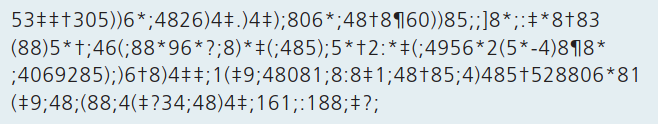
\includegraphics[width=\linewidth]{Figuras/cripto-msg.png}

\textbf{Tarefa}: Crie um algoritmo (em qualquer linguagem ou pseudocódigo) que faça a criptoanálise do texto acima e descubra a mensagem original. 

\end{document}

